\makeatletter
\def\BState{\State\hskip-\ALG@thistlm}
\makeatother

\section*{Monte Carlo Simulation}

Measured 3-$\gamma$ from ortho-Positronium decay count only a fraction of the whole 3-$\gamma$ decay yield. This is due to the fact that the triple coincidence is between detectors at 120$^\circ$. In order to get a correct estimated of the total 3-$\gamma$ events generated by Orthopositronium decay a Monte Carlo Simulation is used. The aim of the simulation is to numerically estimate the ratio:
\begin{equation*}
R_3 = \dfrac{\#\text{eventi 3}\gamma\text{ emessi a 120}^\circ}{\#\text{eventi 3}\gamma}
\end{equation*}

The simulation code\footnote{\noindent The code is available at:\\ \href{https://github.com/LucaMors/Physics_Lab_Reports/tree/master/Positronium/Analysis/Simulation}{github.com/LucaMors/Physics\_Lab\_Reports/tree/master/Positronium/Analysis/Simulation}} is built by three main part:
\begin{enumerate}
\item Event Generator
\item Experimental Setup
\item Run Manager
\end{enumerate}

\subsection*{Event Generator}

The event generator handle the photon creating from ortho-positronium decay. The algorithm used for event creation is the following:
\begin{algorithm}
\caption{Ortho-Positronium Decay Photon Generator}\label{euclid}
\begin{algorithmic}[1]
\State Sample the theoretical energy distribution, $F(k)$ of photon from o-Ps decay the energy for the first photon is obtained.
\State Sample a random point on a sphere surface for the purpose of obtaining the direction for momentum versor.
\State Scaling momentum vector according to the sampled energy.
\State Repeat 1-3 for the 2$^{nd}$ gamma.
\State By imposing momentum conservation obtain the 3$^{rd}$ gamma momentum vector.
\State From previously obtained vector get energy.
\State Sum the energy of all of the three gammas and check if energy conservation holds. If yes return the three Photon object otherwise return to 1.
\end{algorithmic}
\end{algorithm}

The theoretical energy distribution used for the purpose of obtaining photons energy is reported in \cite{ore1949three}.

\subsection*{Experimental Setup}

This part of code handle detector creation and positioning. A detector object is defined by a position vector $\vec{P_d}$ and by a edge vector $\vec{P}_{\text{edge}}$ that point to point belong to detector face edge and is completly determined by the detector face radius (we are considering cylindrical detectors). In order to check if an emitted $\gamma$ impiges onto a detector the code check if the angle ($\alpha_\gamma$) between $\vec{P}_d$ and $P_\gamma$ ($\gamma$-ray momentum) is lower than the half-aperture ($\varphi$) of the cone defined by our detector ( that is the angle between $\vec{P}_d$ and the edge vector $\vec{P}_{\text{edge}}$) as sketched Fig. \ref{Fig: angle det check}.

\begin{figure}[H]
\centering
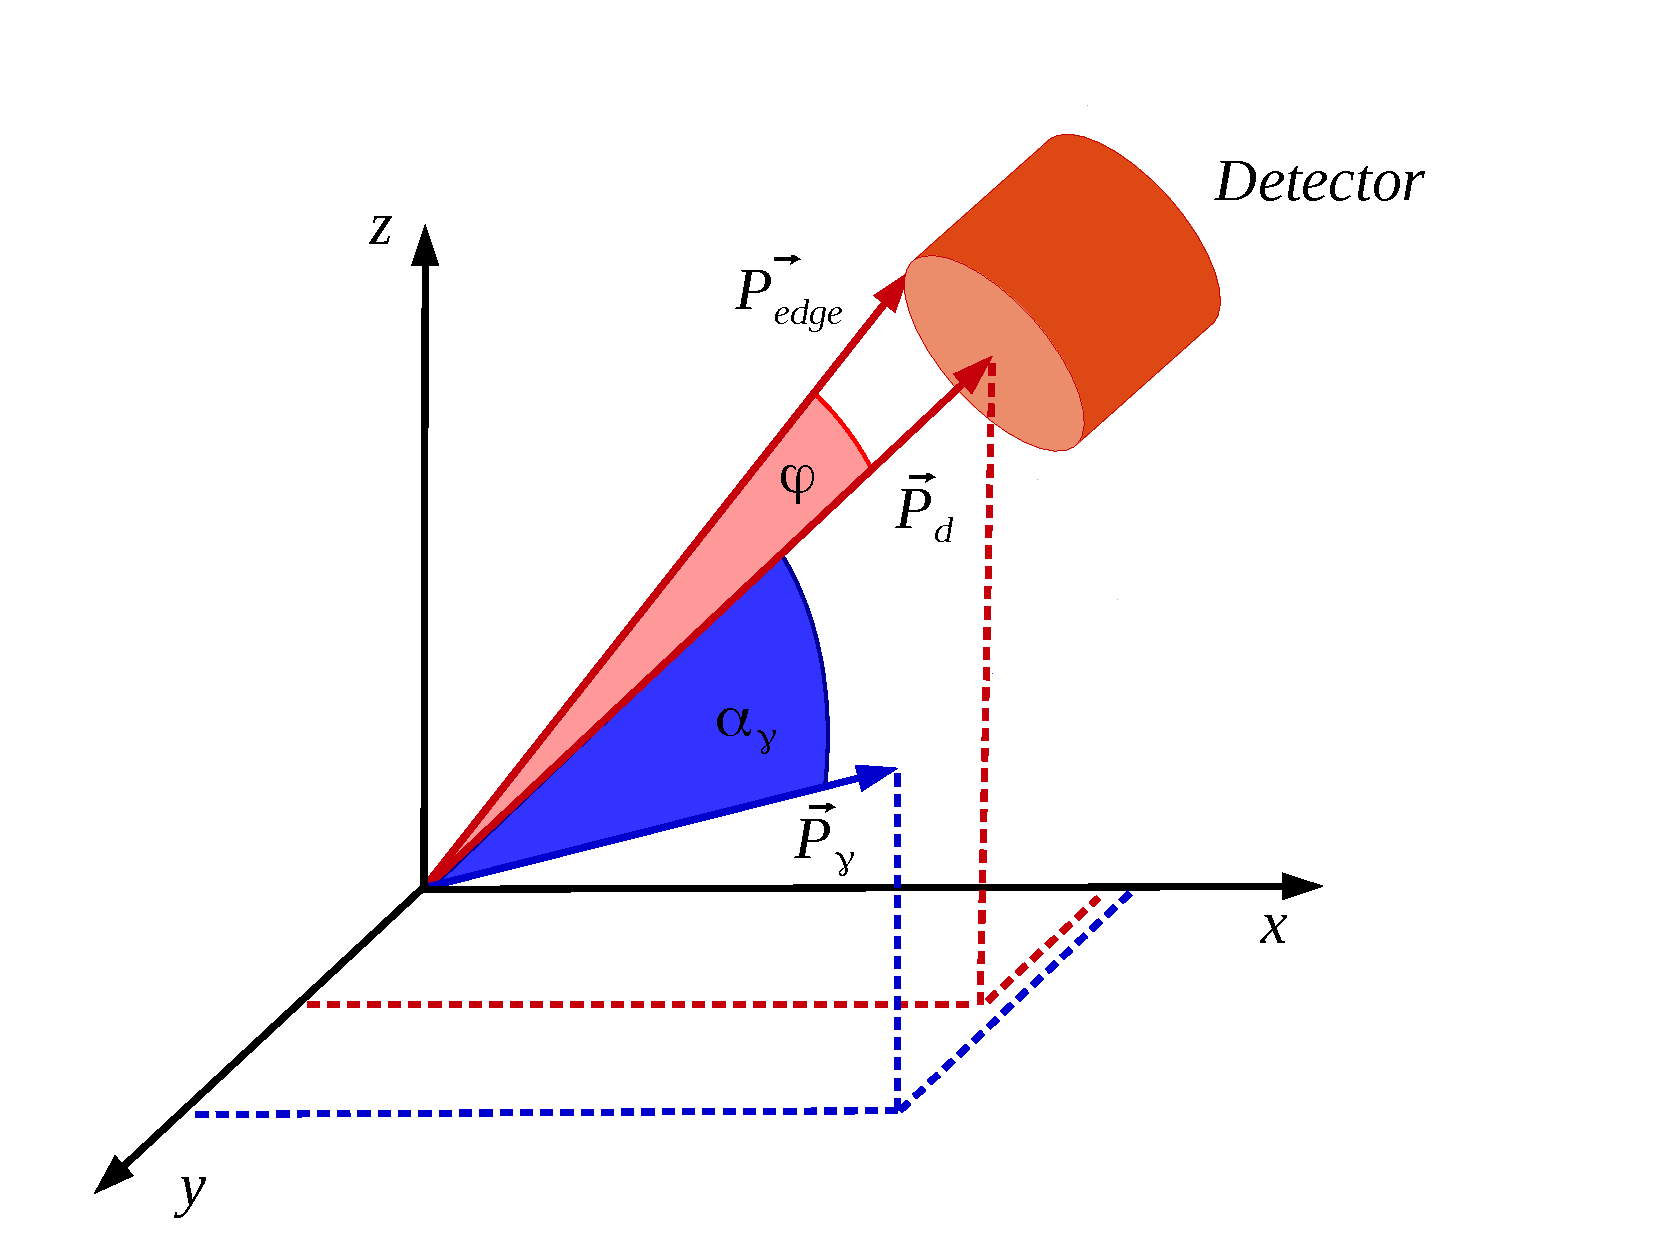
\includegraphics[width = 0.7\textwidth]{check_detector}
\caption{Detector and $\gamma$ angle notation. The situation presented in this figure is that of a rejected gamma.}
\label{Fig: angle det check}
\end{figure}


\subsection*{Run Manager}

This last part of the code handle the coincidence between detectors and the extraction of physical interest plot and quantity.

Using the implemented code a simulation of $10\times 10^6$ events was done and the relevant plots are presented in Fig. \ref{Fig: simulation result} and Fig. \ref{Fig: simulation phi dist}.

\begin{figure}[H]
\centering
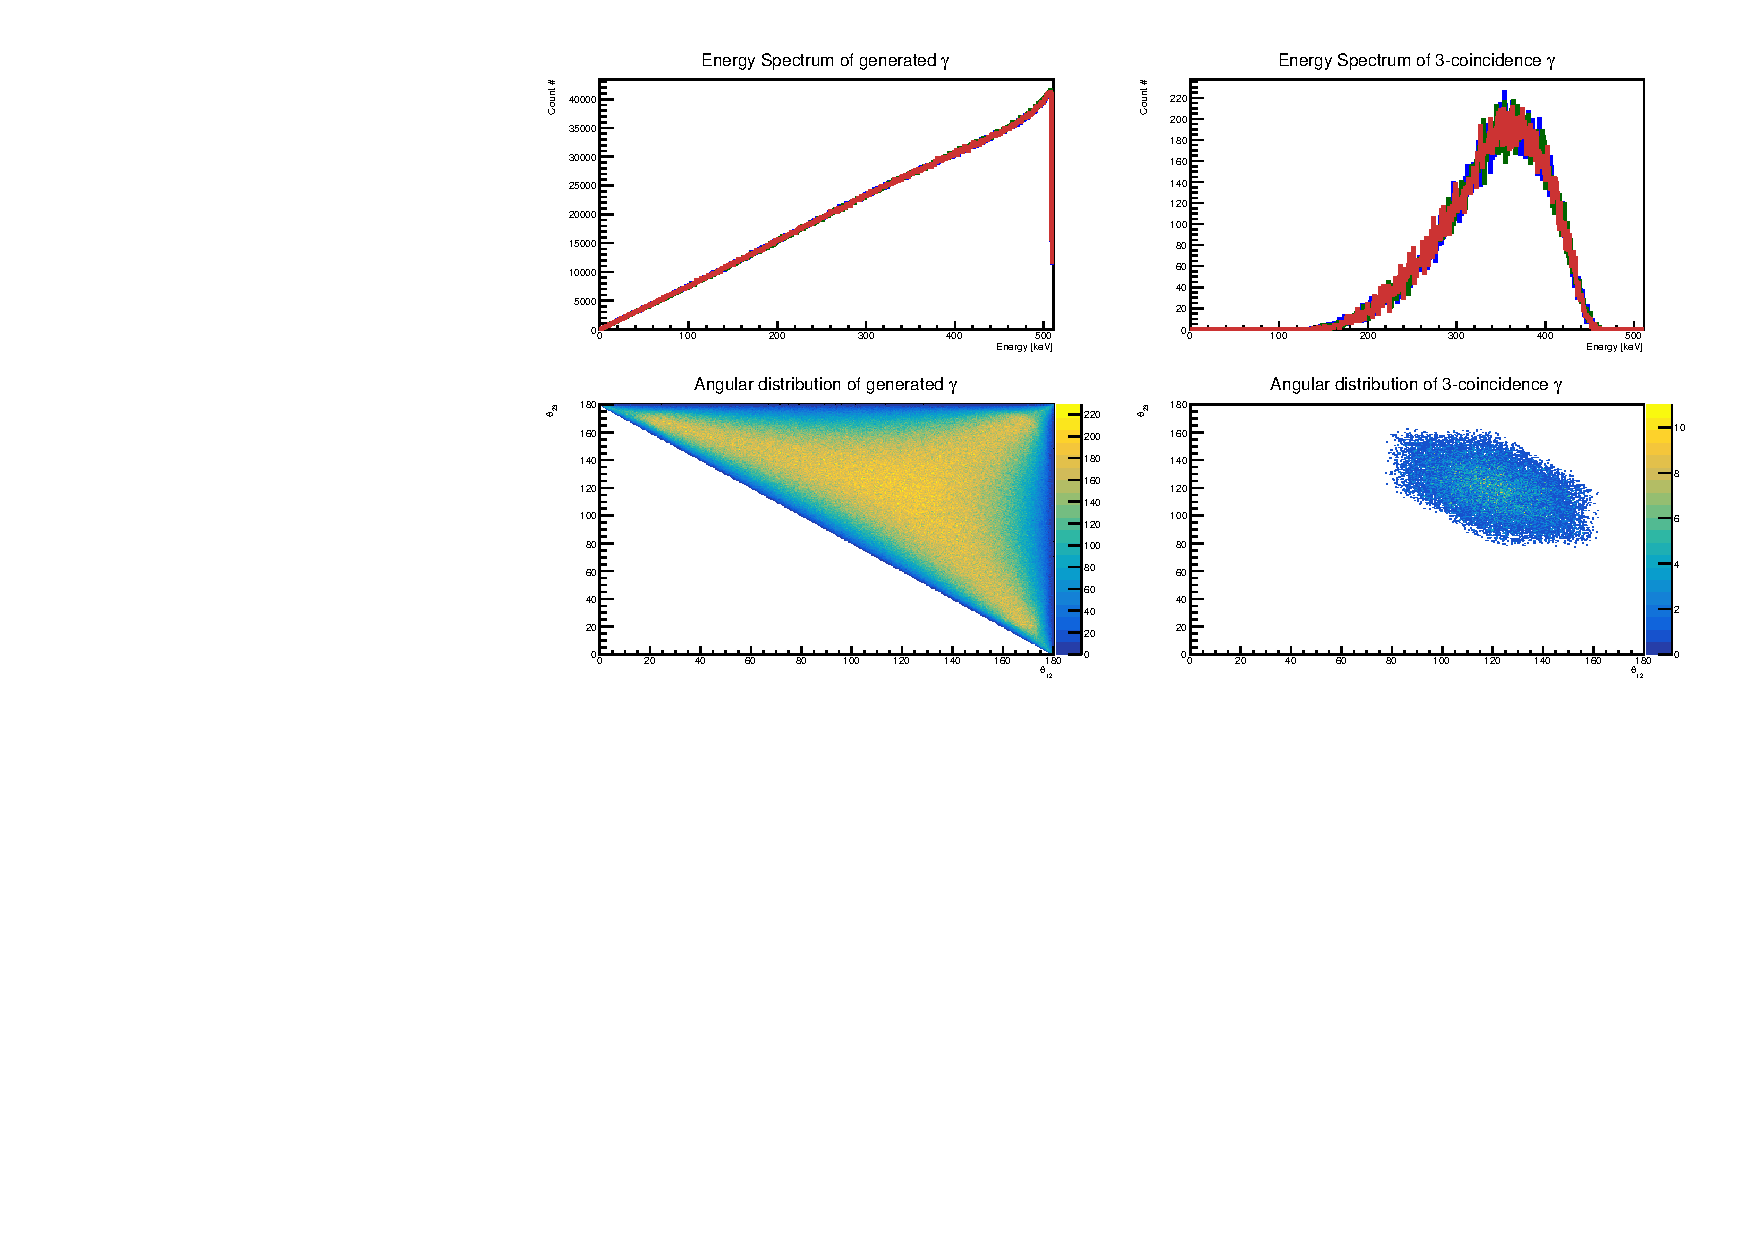
\includegraphics[width = \textwidth]{result}
\caption{(a) Theoretical Energ distribution of genereted gamma. (b) Energy spectrum of the 3-coincident $\gamma$ events. (c) Angular distribution of generated events. (d) Angular distribution of 3-coincident $\gamma$ events.}
\label{Fig: simulation result}
\end{figure}
\begin{figure}[H]
\centering
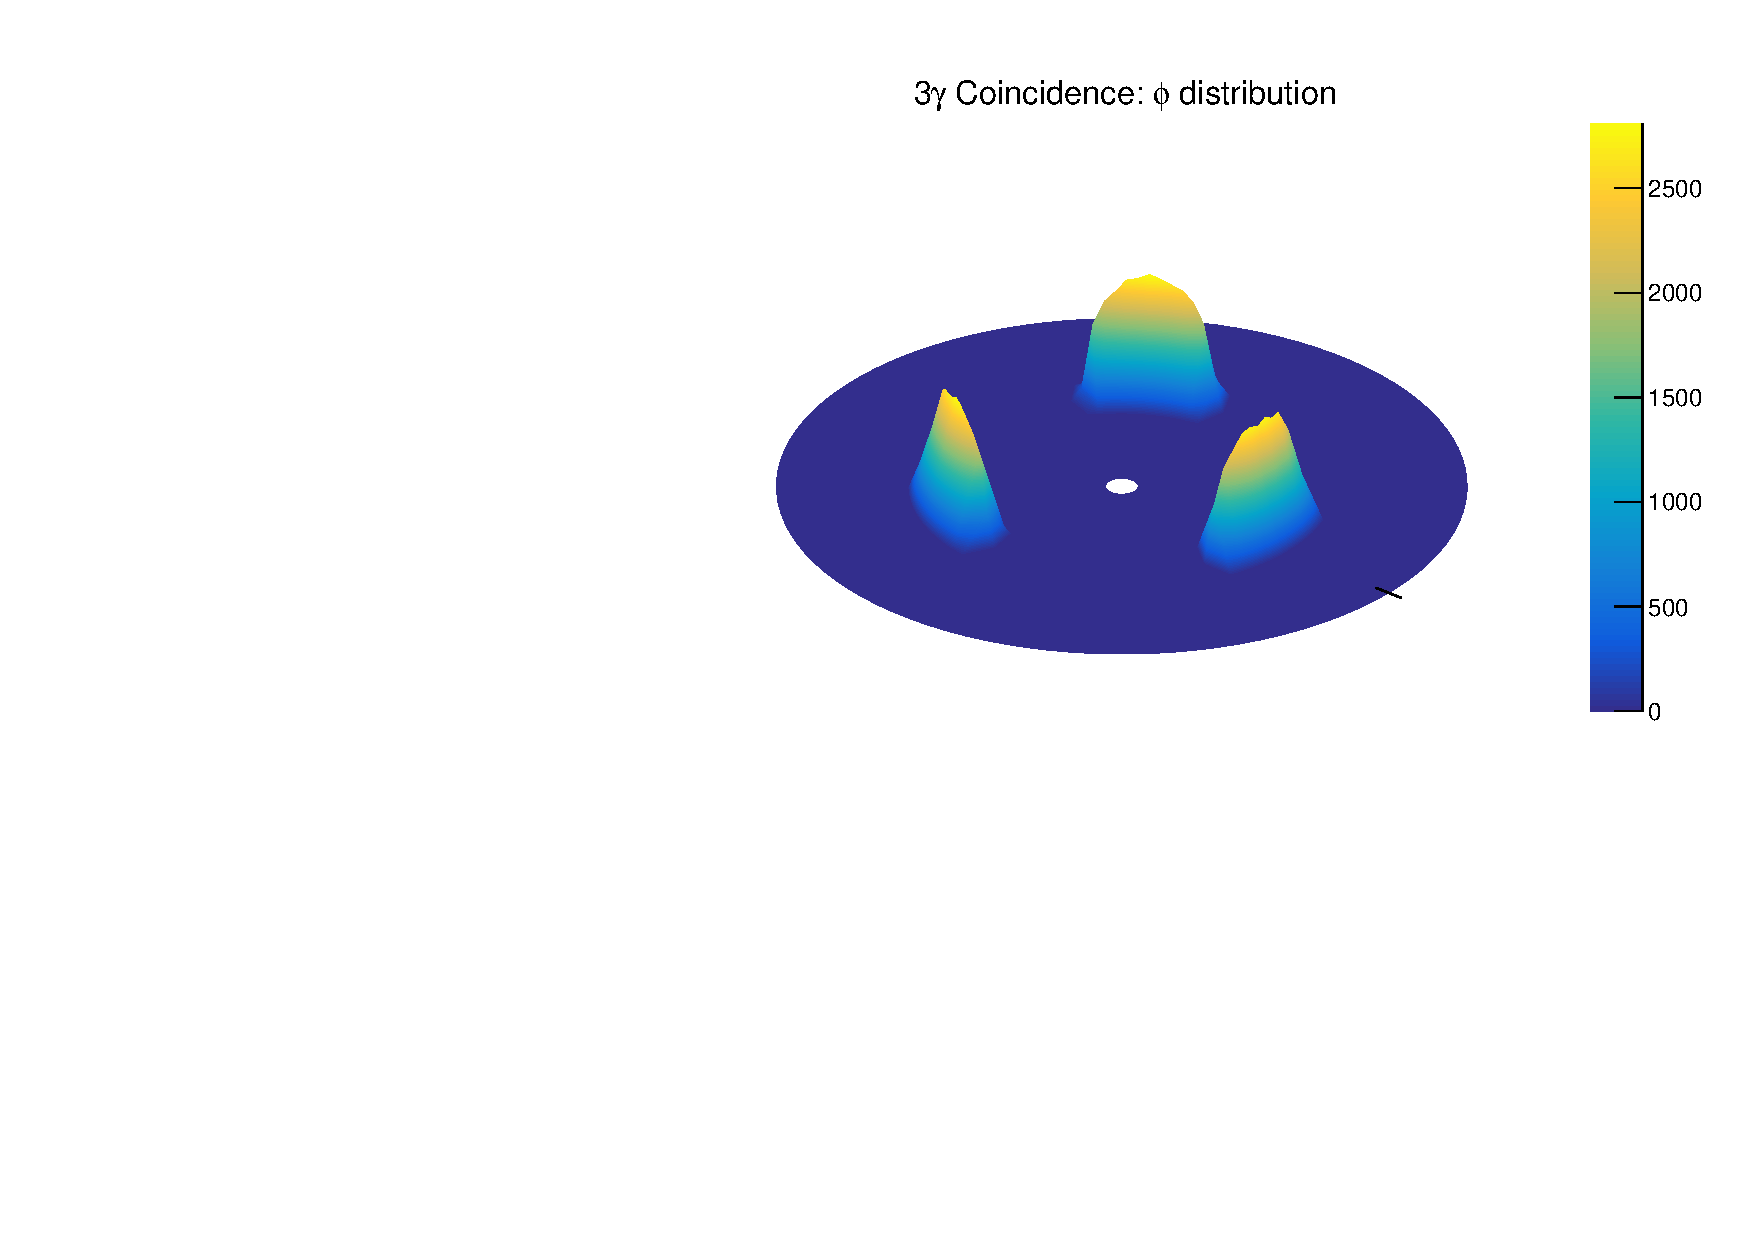
\includegraphics[width = 0.8\textwidth]{3g_phi_dist}
\caption{$\phi$ distribution of coincident events.}
\label{Fig: simulation phi dist}
\end{figure}
